%\documentclass{beamer}
\documentclass[handout]{beamer}

\usepackage{amsmath}
\usepackage{tikz}
\usepackage{commath}

\graphicspath{{figures/}}
\DeclareGraphicsExtensions{.pdf,.png,.jpg}

\usetikzlibrary{arrows,shapes}

\newcommand{\ev}[1]{\langle #1 \rangle} % expectation value

\title[Quantum GI]
{Distinguishing graphs with a quantum annealer
  using susceptibility measurements} 

\author[Wittmann, Hen, Young]{%
  Matthew~Wittmann\inst{1} \and
  Itay~Hen\inst{2} \and
  A.~P.~Young\inst{1}
}

\institute[UCSC and ISI]
{
  \inst{1}%
  Physics Department\\
  University of California, Santa Cruz
  \and
  \inst{2}%
  Information Sciences Institute\\
  University of Southern California
}
\date[APS MM 2014]{APS March Meeting, 2014}

\begin{document}

% Don't show "Figure:" in captions
\setbeamertemplate{caption}{\insertcaption}

% TikZ commands needed for fancy equation annotation
% see http://www.texample.net/tikz/examples/beamer-arrows/
\tikzstyle{every picture}+=[remember picture]
\tikzstyle{na} = [baseline=-.5ex]
\everymath{\displaystyle}

\frame{\titlepage}
\section{Background}
\begin{frame}
  \frametitle{Graph Isomorphism (GI) Problem}
  Are two graphs really the same apart from the labeling of the vertices?
  \vskip -0.5cm
  \begin{columns}[b]
    \column{0.27\textwidth}
    \begin{figure}
      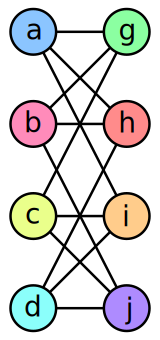
\includegraphics[scale=0.36]{Graph_isomorphism_a}
      \vskip 1cm
      \caption{$G=(E_G,\,V_G)$}
    \end{figure}

    \column{0.27\textwidth}
    \begin{figure}
      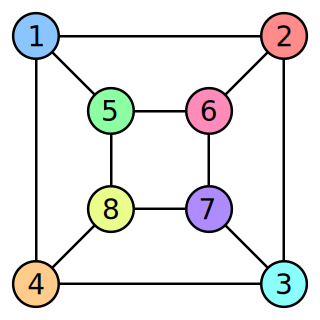
\includegraphics[scale=0.36]{Graph_isomorphism_b}
      \vskip 1cm
      \caption{$H=(E_H,\,V_H)$}
    \end{figure}

    \column{0.27\textwidth}
    \begin{figure}
      \abovedisplayskip=0pt
      \abovedisplayshortskip=0pt
      \begin{align*}
        f(a) &= 1 \\
        f(b) &= 6 \\
        f(c) &= 8 \\
        f(d) &= 3 \\
        f(g) &= 5 \\
        f(h) &= 2 \\
        f(i) &= 4 \\
        f(j) &= 7
      \end{align*}
      \caption{$f:V_G \longrightarrow V_H$}
    \end{figure}
  \end{columns}
\end{frame}
\begin{frame}
  \frametitle{Graph invariants}
  E.g.
  \begin{itemize}
    \item number of vertices and edges
    \item degree distribution
    \item spectrum of adjacency matrix
    \item \ldots and many more (any quantity which is invariant under
      relabeling the vertices)
  \end{itemize}
  \begin{definition}
    An invariant $I$ is \alert{complete} if $I(G) = I(H) \iff G \cong H$.
  \end{definition}
  There are no known general, complete invariants. Finding one would provide an
  easy solution to the GI problem!
\end{frame}
\begin{frame}
  \frametitle{Features of the GI Problem}
  \begin{itemize}
    \item Special cases (i.e. those for which complete invariants can be
      defined) can be solved efficiently by classical algorithms
    \item But the best known general algorithms are exponentially complex in
      the number of vertices
    \item Complexity class \alert{NP}, but unlikely to be NP-complete (the same
      is believed of factoring)
  \end{itemize}
\end{frame}
\begin{frame}
  \frametitle{Physical studies of the GI problem}
    \begin{columns}
      \column{0.5\textwidth}
      \begin{itemize}
        \item Rudolph (2002):
          Exploit physical intuition to construct graph invariants
        \item Hen and Young (2012):
          Propose that the Graph Isomorphism problem could be solved using a
          quantum annelear
        \item Gaitan and Clark (2013):
          Propose adiabatic quantum algorithm for GI
        \item Vinci et al. (2013):
          Carry out first experiment using D-Wave One quantum annealer
      \end{itemize}
      \column{0.5\textwidth}
      \includegraphics{d_wave_one_system}
    \end{columns}
\end{frame}
\begin{frame}
  \frametitle{Co-Ising graphs}
  Encode graph $G=(V,\,E)$ as an Ising Hamiltonian $H(G)$
  \begin{itemize}
    \item 1-1 mapping of vertices to Ising spins
    \item<2-> \alert{Antiferromagnetic} interaction between spins $\sigma_i$
      and $\sigma_j$ for each edge $(i,\,j) \in E$
      \tikz[na]\node [coordinate] (n1) {};
  \end{itemize}
  \begin{equation*}
    \onslide<2->{ % only show AFM term starting on slide 2
      H(G) = 
      \tikz[baseline]{
        \node[fill=blue!20,ellipse,anchor=base] (t1)
        {$\sum_{(i,\,j) \in E} \sigma^z_i \sigma^z_j$};
      }
    }
    \onslide<3->{ % only show field term starting on slide 3
      -
      \tikz[baseline]{
        \node[fill=red!20,ellipse,anchor=base] (t2)
        {$h \sum \sigma^z_i$};
      }
    }
  \end{equation*}
  \begin{itemize}
    \item<3-> \alert{Longitudinal field} to break symmetry
      \tikz[na]\node [coordinate] (n2) {};
  \end{itemize}

  % Draw edges from bullet points to terms (note 'overlay' style).
  \begin{tikzpicture}[overlay]
    \path[->]<2-> (n1) edge [out=0,in=90] (t1);
    \path[->]<3-> (n2) edge [out=0,in=-90] (t2);
  \end{tikzpicture}

  \begin{definition}<4>
    $G_1,\,G_2$ \alert{co-Ising} $\iff$ $H(G_1)$, $H(G_2)$
    co-spectral for all $h$
  \end{definition}
\end{frame}
\begin{frame}
  \frametitle{Adiabatic Quantum Computation (AQC)}
  \begin{itemize}
    \item Driver Hamiltonian
      \tikz[na]\node [coordinate] (n3) {};
  \end{itemize}
  \begin{equation*}
    H = (1-s)\,
    \tikz[baseline]{ \node[fill=blue!20,ellipse,anchor=base] (t3) {$H_d$}; }
    + s\,
    \tikz[baseline]{ \node[fill=red!20,ellipse,anchor=base] (t4) {$H_p$}; }
  \end{equation*}
  \begin{itemize}
    \item Problem Hamiltonian
      \tikz[na]\node [coordinate] (n4) {};
  \end{itemize}
  \begin{enumerate}
    \item Prepare system in ground state of $H_d$ (easy).
    \item Take $s$ from 0 to 1 \alert{slowly}. According to the adiabatic
      theorem, the system will remain in the instantaneous ground state
      througout the evolution.
    \item Ground state of $H_p \longrightarrow$
      solution of optimization problem
  \end{enumerate}
  \begin{tikzpicture}[overlay]
    \path[->] (n3) edge [out=0,in=90] (t3);
    \path[->] (n4) edge [out=0,in=-90] (t4);
  \end{tikzpicture}
\end{frame}
\begin{frame}
  \frametitle{Adiabatic quantum algorithm for GI}
  \begin{itemize}
    \item \alert{Ising antiferromagnet} problem Hamiltonian
    \item Transverse field driver Hamiltonian
  \end{itemize}
  \begin{equation*}
    H = (1-s) \frac{1}{2} \sum \sigma^x_i
    + s \left(
    \sum_{(i,\,j) \in E} \sigma^z_i \sigma^z_j
    - h \sum \sigma^z_i
    \right)
  \end{equation*}
  \begin{itemize}
    \item Conjecture: \alert{Measurements of the ground state should
      distinguish non-isomorphic graphs.}
    \item But the \alert{ground state of $H_p$ is insufficient} to distinguish
      all pairs of graphs (e.g. co-Ising)\ldots
    \item Solution: Take measurements not just at $s=1$, but in the
      \alert{quantum regime}, $0<s<1$
  \end{itemize}
\end{frame}
\begin{frame}
  \frametitle{Numerical work}
  \begin{itemize}
    \item Exact diagonalization using conjugate gradient
  \end{itemize}
\end{frame}
\begin{frame}
  \frametitle{Measurements}
  \begin{itemize}
    \item Energies $E=\ev{H(G)}$, $E_G=\ev{H_p(G)}$
    \item Magnetizations $m_z$, $m_x$
    \item Spin glass overlap
    \begin{equation*}
      Q_2 = \frac{1}{N} \sqrt{
        \sum_{i,\,j} \del{
          \ev{\sigma^z_i \sigma^z_j} -
          \ev{\sigma^z_i} \ev{\sigma^z_j}
        }^2
      }
    \end{equation*}
    \item Analagous quantity in terms of susceptibilities is measurable on the
      D-Wave machine:
    \begin{equation*}
      Q_2' = \frac{1}{N} \sqrt{\sum_{i,\,j} \del{\dpd{\ev{\sigma^z_i}}{h_j}}^2}
    \end{equation*}
  \end{itemize}
\end{frame}
\begin{frame}
  \frametitle{Test case: small co-Ising graphs}
  \begin{itemize}
    \item Study pair of 13-vertex co-Ising graphs $G_{13}$ and $G_{13}'$
    \item Found to be difficult to distinguish by Vinci et al.
  \end{itemize}
\end{frame}
\begin{frame}
  \frametitle{Results}
  \framesubtitle{Absoulte value of difference between $G_{13}$ and $G_{13}'$}
  \includegraphics[width=\textwidth]{delta-grid}
\end{frame}
\begin{frame}
  \frametitle{Future work}
\end{frame}
\end{document}
